\setcounter{chapter}{ 27 }
\chapter{\textbf{``Terminus Rising'', part 2} }


\subChapterTitle{``A Shocking Lack of Violence''} 

\deets{Suko}{July 23rd, 2014}



A rather shocking lack of people getting punched in the face, even when well deserved.  And an even more shocking display of actual diplomatic maneuvering from all members of the team.


\jumpHeadline{Terminus}




\textbf{{[}9 Tokens in the pool{]}}


\sceneHeadline{Mr. Langdon's Apartment}

Mr. Langdon turns away briefly and then turns back to look us up and down consideringly.  He stands and instructs, ``Follow me'' and walks over to a door in the back of the room, leaving the box on the table (he never touches it).  He leads us down a fairly winding set of corridors until he reaches a room with only a single door.  The room is very austere and contains only a desk, a round table and some chairs.  There are some papers and books in the room.



Jaya sits down in the seat facing the door before Hayley can stop her.  Jonah watches Hayley and doesn't sit until she does (which is after Mr. Langdon seats himself).



Mr. Langdon addresses us again, ``What do I need to know?''

``You need to know your enemy,'' says Jonah.

``And who is this enemy?'' asks Mr. Langdon.

``That's not important at the moment, what is important is what your son did-''

``Where did you go to school?'' interrupts Mr. Langdon.  Jonah names some nice-but-not-great school, one that a reasonably talented National might attend.

``So tell me.  What is it, exactly, that he did?'' Mr. Langdon asks, referring to Oliver.

``He reported to me,'' says Jaya.

``He's a decorated officer and killed many enemy soldiers.  He was a very dedicated sniper, and he had insights that gave him a great advantage. His background as a Citizen allowed him to manage risk in a way that others could not,'' elaborates Jonah.

``And do you have any proof of this?'' asks Mr. Langdon.

Jaya and Jonah tell Hayley to give Mr. Langdon the papers.  Hayley does so, saying that they were prepared for Mr. Langdon's Filis.

Mr. Langdon reads the papers and Jonah watches him closely to see what parts of the papers he pauses at.  {[}\textit{Challenge 1:  Notice what catches Mr. Langdon's eye. Business Contacts 2 (Jonah) $\rightarrow$ Overcome! }\textit{\textbf{1 VP (Jonah)}}{]}.  Mr. Langdon pauses when he gets to the sections on cause of death (asphyxiation from enemy inflicted wounds) and at the listing of Oliver's rank.  He seems to be searching for something... some sort of proof of something.

``My apologies if I say anything inappropriate, but we only know what we know because of your son's sacrifice,'' says Jonah.

Jaya coughs and asks for a drink.  Mr. Langdon suggests using their canteens.  Hayley hesitates and then unslings her rifle to \hl{rummage through her backpack}\footnote{\textbf{Nathaniel Ford }For future reference, canteens are probably easily accessible, second only to weapons and ammo.

Also, in this vein, that pack is pretty hefty. It would prohibit sitting in chairs easily. Should have noted this sooner. \textsubscript{07/28/14 6:47pm}}\footnote{$\rightarrow$\textbf{Suko T }Yeah I had assumed she probably had to take off her backpack and unsling her rifle to sit down.  Jonah and Hayley are already in combat armor which is going to make sitting in most civilian chairs somewhat...difficult already :)  I figured Hayley's canteen is only easily accessible if someone like Jari taught her how to pack the backpack correctly, otherwise it was probably tidily tucked away somewhere where it wouldn't get dented or knocked around.  Unless taught otherwise, she packs like a Citizen, not a soldier.  Except for her weapons and ammo.  You better bet those are right at hand. :D \textsubscript{07/28/14 11:05pm}}to pull out her canteen and offers it to Jaya.  Jaya frowns a little at Hayley but takes a swig and hands it back.  While this is going on, \hl{Mr. Langdon goes to the desk and pulls a thin cord}\footnote{\textbf{Nathaniel Ford }I forget the exact dialogue, but there was some mention of the vote or asking him for something that preceded this. \textsubscript{07/28/14 6:48pm}}.

``Have you visited Terminus often?'' asks Mr. Langdon.

``No,'' says Jonah.  Jaya says nothing.  Hayley nods but says nothing.

The door opens and Jaya goes on alert.  Hayley, in the middle of putting the canteen back, puts her hand on her rifle and watches the door alertly.  A small, slight woman in plain robes (not house livery) walks in.  She looks slightly surprised, as if she was not expecting there to be other people in the room.  She turns to Mr. Langdon, ``How may I assist you sir?''

``The usual,'' he replies and she nods and goes to stand to one side next to the wall.  Hayley takes her hand off her rifle and relaxes.  Jaya is looking suspiciously at the woman.  Hayley leans over and whispers quietly in Jaya's ear, ``This is a Fili, used to record any official conversation.''

``Please continue,'' says Mr. Langdon with a gesture.

``Do you know about Operators and Agents, sir?  How they work?'' says Jonah.

``Why don't you explain it to me?''

``Agents are the hands- they engage with immediate threats.  Operators are more about long term strategy.   I wanted you to understand this because Oliver was an Operator and he noticed something about the enemy.''  Jonah pauses and then asks, ``I assume you know about Nicklepan?''

``Perhaps.  Why don't you tell me what you know about it?''

``Through fighting the enemy-''''

``This nameless enemy?'' interjects Mr. Langdon.

``-Operator Langdon was able to notice something about how the enemy worked.  They are extremely dangerous'' says Jonah.  

``Is that so?  Is that the important information?  And what am I expected to do with this?''

``There is a senate vote approaching,'' says Jonah.

``I will not discuss such things with you.  I've never met you.  I don't even know who sent you, or even if you are who you say you are,'' says Mr. Langdon.  Hayley is looking alarmed and opens her mouth to say something, then shuts it.

Jaya makes a frustrated noise and rubs her nose.  ``Let's get to the point,'' says Jaya.  Hayley looks horrified.  {[}\textit{Challenge 2:  Notice.  Stash 2 (Jaya) $\rightarrow$ Matched{]}}.  Jaya's perception is sharpened by the drugs she just took, Jaya can tell \hl{that Mr. Langdon doesn't believe us}\footnote{\textbf{Suko T }I think this is what she noticed?  Yes? \textsubscript{07/27/14 10:52pm}}\footnote{$\rightarrow$\textbf{Nathaniel Ford }It probably went beyond that to, ``Mr. Langdon did not find you believable/credible.'' \textsubscript{07/28/14 6:50pm}}.

Mr. Langdon says in a voice full of controlled anger, ``Yes. By all means, let us get to the point.  Let me see if I can summarize this.  It seems like you want me to know my son is dead.  And the people who did it are some nameless enemy that I have to take your word for is dangerous.  I am to keep this in mind at the next senate meeting.  Is that all?''  Mr. Langdon stands and rests his hands on the table.  ``If you what you claim is true, and you aren't a bunch of grenadiers trying to shake me down for...whatever it is you are trying to shake me down for, then we are done here.''  He leaves the room.  Hayley is looking almost ill with distress.  Jaya leaves.  Jonah pauses turns to the Fili.  ``I would like to state for the record that we extend our condolences for the loss of Operator Langdon.  \hl{We came here to inform his father of his son's dedicated service.}\footnote{\textbf{Suko T }I think there was something else that Jonah added to the message about the vote or something but I have no notes on what it was. \textsubscript{07/25/14 2:58am}}````I cannot convey messages sir,'' says the Fili politely.

``That's okay, I just want it to be part of the official record.''

``If I am asked to repeat the record, I will repeat these words.''

``Very good.  Thank you,'' says Jonah.  The Fili looks uncomfortable at the thanks.

Hayley waits until Jonah is leaving the room and then nods at the Fili with the precise level of respect due to her position and follows Jonah.  Jaya and Hayley keep an eye out for the butler as they leave but do not see him.  {[}\textit{Challenge 3: Notice what was up with Mr. Langdon.  Process Wonk 2 (Hayley) + Nose for Breadcrumbs 2 (Hayley) $\rightarrow$ Matched{]}}. As they walk out, Hayley slowly puts together the bits of information she was gathering about Mr. Langdon.  She realizes that Mr. Langdon was fishing for information from us.  He was under some sort of pressure from someone, a pressure that is forcing him to do something.  He didn't know if we were part of that group or some new party trying to manipulate him.  He felt like we were shaking him down for something but he didn't know what.



\textbf{{[}3 Tokens remaining{]}}



We leave the apartments.  Jonah turns to Hayley and says with an exasperated edge to his voice, ``Okay what is that you wanted to say in there?''

Hayley still looks upset and says, stuttering a bit, ``W-Why did you do that? Why did you- you- say such things?  How could you insult him like that?  Why- why didn't you want us to succeed at our mission?''

Jonah sounds frustrated.  ``Explain.  What should we have done?''

``Answer his questions!  He was looking for answers.  He needed something to help him.  He's \hl{under some sort of pressure}\footnote{\textbf{Suko T }I feel like Hayley suggested that we warn Mr. Langdon about his butler, but I can't figure out where that might have come up. \textsubscript{07/25/14 3:32am}}.  We could have told him the name of-'' Hayley looks around, realizes they are on the street and amends, ``-er, the thing we shouldn't say in public.''

``Let's go somewhere where we can talk,'' says Jonah and we all troop off to Terminus Station.



Jaya commandeers a private office room from a junior TA agent and they close the door.  Jaya sits down but clearly is indulging the other two and doesn't seem very interested in this conversation.

``Now, tell us what you wanted to say but couldn't before,'' says Jonah to Hayley.

``Octavius.  Give him the name.  Wasn't that the point?  To tell him about Octavius?''

``We \textit{did} tell him.''

``But a name, we didn't give him a name.''

``When did he ask for a name?''

``When he said 'this nameless enemy'''

``And I was supposed to know that meant he was asking for a name?''

``Well yes, when a Citizen repeats something like that it generally means that they want to know the answer.''

``Why would he care what the name is?'' asks Jonah.

``Because Citizens care about names, names are important to them,'' replies Hayley.

``Oh, like street names?'' asks Jaya.

``Um...yes?  I think so.  I don't think they use those kinds of names but names are powerful.  Like family names,'' says Hayley.

``We had no proof, why would giving him a name have helped?'' asks Jonah

``Because it would have given him a focus, something to work with. He was looking for something from us.''

``I don't think it was going to matter, he wasn't going to listen to us anyway,'' says Jaya.

``But he was!'' protests Hayley.  ``He took us to that second room.  That meant that he was taking us seriously enough to want the conversation to be private, where the servants would not overhear it.  And he requested a Fili, which meant he wanted it recorded so it would be an official conversation.  He was being respectful.''

``Really?  It didn't look like it.  It was a pretty shitty room.  He didn't even offer us a drink!'' says Jaya.

``Exactly!  If he had offered us a drink, it would have been a social call and nothing could be taken seriously,'' says Hayley.

``How were we supposed to know that?'' says Jonah, starting to sound angry.

``You didn't?'' says Hayley, confused.

``No.  We didn't,'' says Jonah flatly.

``But I thought everyone knew that.''

``No, everyone doesn't.  We don't know any of this, Hayley, we're not Citizens.  We don't know this kind of thing.''

``Oh.''

``That's why you needed to tell us.  If you knew we were saying the wrong things, you should have said something.''

``But how was I to know you didn't know it?  \textit{I} knew it, and I don't know very much at all, so I assumed everyone knew these things.''

``Hayley, you know lots of things we don't know, especially about all of this.''

``Oh.  But- but- how am I supposed to know what you don't know?''

``You need to let us know when we are offending someone, some sort of signal-''

``You can cough!'' volunteers Jaya.

``Or whisper it to us discreetly,'' says Jonah.

``Okay...'' says Hayley dubiously. ``But if I'm seen as guiding you, it will undermine your authority.''

``Was the fact that I was talking for Jaya a bad thing?'' asks Jonah.

``Um, well I don't know much about military protocol in social situations like that.  It is true that often a Citizen will have a representative speak for them, especially if it's a situation where the wording is important.  They will usually have a Fili recite their prepared words.  But in this case... it was definitely strange.  It made the chain of command unclear.  Especially because we didn't prove to him that we were who we said we were-''

``And how were we supposed to do that?  It's not like we have papers,'' says Jonah. ``How were we to know we'd need anything more than our badges?''

``We- we could have had him contact Station Chief Ogleby, who could have verified our status.  It wouldn't have taken long for his assistant to establish our credentials.''

``Didn't he already know we were sent by the Station Chief?'' asks Jonah.``Probably not.''

``What??  Why did he accept the appointment then?''

``He didn't accept the appointment, his assistant did.''

``And they didn't include any names?'' asks Jaya.

``No, of course it included our names, but why would it have included the requestor's name?''

``Why wouldn't it?''

``Most appointments are set up by assistants, why would he want to know what the assistant's name is?''



Jaya gets bored at this yammering and heads off to talk to Station Chief Ogleby.  She gets a map of where the Senators are, and is told that it is still hard to find Agent Lorentz.  Jaya comes back and Jonah is still grilling Hayley.  



``Tell me what I should have said differently,'' says Jonah intensely, sounding pretty worked up.

``I- I- I don't- um, you said so many things.  What part do you want me to say?'' flounders Hayley, looking and sounding distressed.

``Everything.  All of them.  Start at the beginning and go over everything,'' says Jonah coldly.

``I- Okay- but- I don't remember every word- I'm sorry- I don't know how- I'm not used to talking to Citizens....'' \hl{Hayley is pretty incoherent and looks unhappy.}\footnote{\textbf{Suko T }I probably should have been hyperventilating more but if it didn't come across: this is more than her usual inability to articulate her thoughts.  She seems to actually be panicking a little.  Something about this situation is distressing her on a deep level.

Dealing with the nice, orderly bureaucracy to see Senator Bennett calms her down. :) \textsubscript{07/28/14 4:24pm}}

``Lay off, Jonah,'' says Jaya.  Hayley looks at her gratefully.

``No.  We need to know this.  If Hayley knew how to handle this situation, she needs to tell us what to do, and exactly what to say.''

\hl{``Look, she's not a Fili okay?   You're a big boy, you can come up with your own words,'' says Jaya.}\footnote{\textbf{Suko T }Aww.... protector Jaya! :) \textsubscript{07/28/14 4:25pm}}

``In that case she needs to teach us what she knows about Citizens and protocol,'' says Jonah stubbornly.

``I'm st- I'm not that smart so it took me four months to learn just the basics,'' says Hayley hesitantly.  ``I don't think- I don't think we have that much time-''

``Try,'' says Jonah implacably. 

``I think we're done here,'' says Jaya and she tries to grab Jonah.  Jonah dodges out of the way and Jaya ends up punching a hole in the wall.

``Fine!  Then I wash my hands of all of it.  I won't be dealing with any of this anymore,'' says Jonah angrily.

``You're leaving?'' asks Hayley, alarmed.

``No you're not leaving-'' says Jaya at the same time that Jonah says, ``No, I'm just not going to say anything anymore.  You can take care of all of it.''



It is decided that due to the time pressures, we will split up and tackle the Senators separately.  Jaya says that she'll go with Hayley and see Senator Bennett.  Jonah will go see Senator Marechenko.


\sceneHeadline{Senate Administrative Building}

Jaya starts sweating at just the sight of the building which looks a lot like the one that housed the Security Triumvirate interrogation.  Hayley confidently navigates them through the slow process of getting to see Senator Bennett.  Hayley and Jaya wait in several waiting rooms until they reach a room where a guard asks them for their weapons.  Jaya tries to see if they'll let her keep her truncheon but they won't.  Hayley reluctantly surrenders her rifle, making the soldier nervous with her list of instructions on how to handle it safely.  They also request that Hayley remove her helmet and give it to them.  In the next room, Hayley definite gets some looks from the people waiting there but neither she nor Jaya notice.  A page comes to escort them down a short corridor to a large room.   In the corridor, Hayley does her best to disguise the sweat stains and straighten Jaya's uniform.



\textbf{{[}Senator Bennett Activated. 12 Tokens enter the pool{]}}



Senator Bennett is at a table with lots of papers.  There is a Fili to his left and a big bruiser standing behind him.  There are two other unfamiliar people at the table and four other guards spread out around the room.  Two of them are guarding the door.  There is a second page pouring water into some glasses.  There is no place for Hayley and Jaya to sit.  Hayley follows Jaya to the center of the room and stands slightly behind her and to her left.



``Agent Parvadi, you've come up in the world.  I admit, I'm surprised.  I'd have expected Morgan to come herself.''

Hayley looks at Jaya, and Jaya nods. Hayley turns back to Senator Bennett.  ``I am sorry, that was not going to be possible sir,'' says Hayley calmly.

``And why not?''

``I am not at liberty to say, sir.''

``Really?  Under whose orders?''

``I am not at liberty to say, sir,'' repeats Hayley politely.

``Am I going to have to give you a direct order?''

``I know your time is valuable sir, could we convey to you the important information that we are here to deliver?  And then deal with this matter later?''

``Very well,'' says Bennett.

``There is an important vote approaching, and we have information that will affect it.''

``I assume you are not referring to the sewer tax?'' says Bennett sarcastically.

Hayley pauses to consider the question seriously and then replies, ``I do not know the name of the vote sir, but I believe not.''

``And the order to give me this information was given to you by your commanding officer?'' asks Bennett, fishing for information.

``Yes sir,'' replies Hayley.

``Is your line of command stable?'' asks Bennett.

Hayley pauses, thinks, and then says firmly,\hl{``The order was issued by my standing commanding officer, sir.''}\footnote{\textbf{Suko T }As Nate said, this implies that Morgan is not dead and/or that our command chain is unchanged. \textsubscript{07/27/14 10:58pm}}

``Interesting.   What is the message then?''

``The enemy is not going to negotiate fairly,'' says Hayley after a few false starts to phrase the information.

``Fairly?''

``The enemy will take advantage of any weaknesses and exploit them.''

``So, no peace with Anglia then?''

``I have no opinion on that matter sir, I am just here to convey this information,'' says Hayley calmly.

Bennett turns to Jaya and asks her, ``And you have no opinion on this either?''

``Peace with Anglia is a bad idea,'' says Jaya.

``Some people are opposed to war,'' says Bennett.

``Some people are opposed to violence,'' says Jaya.  ``But sometimes it is necessary.''

Bennett looks skeptical.

``The enemy has unorthodox tactics and they will kill everyone,'' says Jaya.

``I'm sure Morgan believes that,'' says Bennett.

``We are here because we witnessed it, sir,'' says Hayley.

``Yeah we were at, uh,'' says Jaya, looking at Hayley for a prompt.

``Nicklepan and Borroughs,'' supplies Hayley.

``Yeah those places.  We saw the bodies.  Negotiation is going to fail.  Resistance is likely to succeed,'' says Jaya.

``Interesting that you don't mention Transit Minor,'' says Bennett.

``We were not there, sir.  We cannot report on what happened there,'' says Hayley.

``You seem remarkably uninformed,'' says Bennett and make a small gesture.

The guards move to stand in front of the door.  Jaya turns around to watch them.  Hayley doesn't even turn around and keeps watching Bennett steadily.

``I would like to take this off the record,'' says Bennett.

Hayley turns her head to look at the Fili.  Bennett sighs and then dismisses the Fili who leaves the room.  Jaya is tense.  Hayley is relaxed.

``Now that we are off the record, let me ask you a question.  How many of your comrades have you lost?''

Hayley scrunches up her face as she appears to be thinking and counting.

``Just one, technically,'' says Jaya.

``Was that hard?  You lost a quarter of your team.  You really want us to fight these people?''

``Yes because otherwise we lose all of us,'' says Jaya.

``Are you sure you won't die either way?'' asks Bennett.

``We are soldiers.  It is our duty to give our lives to protect the Directorate,'' says Hayley.

``And that means you'd protect the Directorate- even over Agent Morgan?'' asks Bennett.

``We work for the TA, who protects the Directorate,'' says Jaya evasively.

``Ah, so if your orders changed, you would follow them?'' prods Bennett.

``We follow our orders,'' says Hayley.

``Oh really?  Hm.''  Bennett leans over to one of the people at the table and talks with them briefly.  The person gets up and picks up some paper and starts filling it out.

Hayley waits patiently. Jaya doesn't say anything either.



The man hands the papers to Bennett who nods and then indicates they should be given to Hayley and Jaya.  The papers are placed on the table in front of them.  ``These are your new orders,'' says Bennett.

Hayley sees Jaya frowning as she peers at the papers.  ``May I read the orders out loud so that everyone is aware of the terms?'' asks Hayley.  Jaya gives her hasty approval and Bennett nods too, smirking.  Jaya and Hayley are being re-assigned to Station Chief Vargas\sout{ \hl{Hassan} }\footnote{\textbf{Suko T }I picked a name so that we didn't keep calling him SC X.  Hassan came from the SC's name from the first version of Borrough Station (before he became Hughes). :) \textsubscript{07/26/14 2:05am}}\footnote{$\rightarrow$\textbf{Nathaniel Ford }Should be someone not Hassan, but I approve of naming this person. \textsubscript{07/28/14 6:51pm}}\footnote{$\rightarrow$\textbf{Suko T }Random name generator sez: Vargas.  Is this the same SC that issued the arrest warrant?  If not, let me know and I'll pick another name for that one too. \textsubscript{07/28/14 11:08pm}} in the regular military, someone that they don't know.  It is a clear demotion.

``These are your new orders.  Sign them,'' says Bennett.

Hayley makes no move toward the paper.  She looks down at the orders and then back up at Bennett.  ``My apologies sir, I cannot sign any legal documents,'' she says solemnly.

``And why not?'' asks Bennett, his smile disappearing.

``I am not legally able to do so, sir.  My apologies,'' says Hayley politely.

``And who can?''

``My contract holder, sir.''

``And who is your contract holder?''

``I am not at liberty to say, sir.'' says Hayley.

Bennett turns to Jaya.  ``And you, are you going to sign the order?''

\jonahBrain{He's bluffing} thinks Jonah at Jaya.

``I've just been promoted, sir and I have grown accustomed to getting a clear picture of what is going on and being informed and having a clear chain of command.  I strongly feel that this order should be cleared with my current commanding officer before moving forward.  I am not comfortable assuming that you have the authority to issue this order.  Could you maybe explain why this order is being made?'' says Jaya, stonewalling brilliantly.  Throughout this speech, Hayley is growing increasingly nervous as she eyes the guards surrounding them.

``Do you \textit{want} to die?'' snaps Bennett, sounding annoyed.

At that Hayley freaks out and spins around to try to put her body between Jaya and the four guards.  Exposed in the middle of the room, she does her best to cover as many angles as possible. {[}\textit{Refresh Bodyguard 2 (Hayley)}{]}  The guards go on alert.

Jaya doesn't move and keeps staring at Bennett.  She replies, ``No.''

``What I mean is that if you don't get out of Morgan's chain of command, you will be executed along with her.''

``If this is all off the record... Octavius is not going to just stop at a few, \hl{she's}\footnote{\textbf{Suko T }I believe this was a deliberate use of the female pronoun. \textsubscript{07/27/14 11:01pm}} going to kill everyone,'' says Jaya and she starts walking forward.

``Do not take another step,'' warns Bennett.  Jaya stops but she glares.

``How droll,'' says the beefy guy standing next to Bennett.

At that, Hayley gasps and immediately abandons guarding Jaya's back and moves to stand between Jaya and the beefy guy.  She looks very worried and tense as she tries to track the movement of everyone in the room.

``If you are intimidated by just this conversation....'' taunts Bennett. {[}\textit{Challenge 3: Don't be intimidated by Bennett.   Left Arm 3 (Jaya) $\rightarrow$ Matched}{]}.

Jaya steps forward again and crosses her metallic arm over her regular one.  The servos on the wrist whirl audibly.   ``DO I LOOK FUCKING INTIMIDATED?'' she demands.  

``This is your last chance.  If you don't cooperate, you will die,'' says Bennett.

``We just want this to be clear.  Don't be Octavius' bitch,'' says Jaya and she starts walking to the door, with Hayley following behind her.Bennett lets them go, waving to the guards to let them pass.  ``One more thing.  Bring a message to Agent Morgan-''

``I'm an Agent,'' says Jaya.  \hl{``Not a fucking courier service.''  She walks through the doors with Hayley and the doors close behind them.}\footnote{\textbf{Suko T }Love this exit. \textsubscript{07/28/14 4:35pm}}



In the hallway, Jaya turns to Hayley and asks in a fierce whisper, ``What the fuck was going on in there?''

``That was clearly an agent of Octavius,'' whispers Hayley, still looking worried.  ``Sir, do we let them live?''

Jaya broadcasts to Jonah  \jayaBrain{We were fucking set up!  He's already working for Octavius.  They tried to fire me!  What the fuck!!??} 

``Is it okay to kill a Senator?'' Jaya asks Hayley.

``We have no standing orders regarding this situation.  But he is already the enemy,'' says Hayley.

``I assume if we kill him, Morgan's going to be upset.''

``Perhaps.  We were only supposed to get them to vote to resist and clearly he will not.''  Hayley looks thoughtful.  ``Though if he's dead, he may not be able to cast his vote.''  Hayley looks at Jaya.  ``What should we do, sir?''

``Do you think we can take them?'' asks Jaya.

``If we had our weapons, possibly.''

``Yeah, we don't have those.  And I think Morgan would be mad about it.''

``Our weapons are only two rooms away, we could get them and return,'' says Hayley calmly.

Jaya thinks hard and then sighs.  ``Nah, we better not.  Morgan'd fucking kill me.''

Jaya and Hayley leave the building without incident and retrieve their weapons and gear without a hitch.  Jaya's tense and jumpy, waiting for an ambush at any moment.  Hayley is alert but seems fairly at ease in the building.



Jaya and Hayley make it to the courtyard and 6 TA soldiers are waiting for them there with rifles.  They all see each other at about the same time.  ``Run!'' says Jaya and she bolts.  {[}\textit{Challenge 2: Outrun the soldiers.  Adrenaline Junkie 2 (Jaya) $\rightarrow$ Matched}{]}.  Jaya escapes down the street.



Hayley runs afterward, but slowly, limping.  Two of the soldiers pass her, and duck into some side streets.  ``Agent Hayley!  Halt!'' calls out one of the soldiers.  Hayley stops and turns to face them. ``Um, I'm afraid I have to arrest you?'' says the constable.

``Under what authority?'' asks Hayley pleasantly.

``Uh, my commanding officer, Station Chief Vargas.''

\hl{Hayley nods and looks at the constable steadily.  ``I see.  You may inform him that you tried.  You may leave now.'' {[}\textit{Challenge 2: Pull Rank.   TA Battle Dress Uniform 2 (Hayley) $\rightarrow$ Matched}{]}.  Hayley unnecessarily straightens her uniform collar and makes sure her Agent badge is visible and smiles nicely at the constables.}\footnote{\textbf{Rebecca S. }sweeeeeeet \textsubscript{07/28/14 10:19pm}}

The constable looks very nervous and says, ``Er.  We saw the suspects and pursued them to, uh....'' he looks around for the street name.  Hayley helpfully gives him the street name.

``...Mulberry street and, uh, lost them.''

``Very reasonable.  Well done,'' says Hayley approvingly and watches as the soldiers withdraw.  Still limping, she jogs to catch up to Jaya, keeping an eye out for the other soldiers that had passed her earlier.

``We should run faster now,'' she tells Jaya.

``Jesus Christ Hayley!  Your leg!  What the fuck is wrong with it?'' says Jaya.

``It is psychosomatic.  \hl{It's all in my head}\footnote{\textbf{Rebecca S. }I like to think that Hayley just accepts and has internalized that she needs to explain all large multi syllable words she might use. \textsubscript{07/28/14 10:25pm}}\footnote{$\rightarrow$\textbf{Suko T }Just doing my job ma'am.  :D \textsubscript{07/28/14 11:13pm}},'' says Hayley apologetically.



\textbf{{[}9 Tokens remaining{]}}



\textbf{{[}Senator Marechenko Activated. 12 Tokens enter the pool{]}}



It is an ornamental house, the neighborhood is more sparsely populated and cleaner, with few people.  In the antechamber, Jonah is offered a drink, but declines.  Jonah is allowed to keep his weapons.  A man approaches him, ``The host would be honored if you would have a drink with him.''



Marechenko is out on a widow's walk, a series of planters along the circuit around the top of the house.\sout{ balcony }\sout{  with a garden }.  He is younger than Bennett, and has slightly lower rank.  Marechenko offers Jonah a glass of whiskey and gestures for him to join him.



``Agent, good to see you!  Sorry for the informality and off the record nature of this conversation, it is important to relax before big senate meetings,'' says Marechenko with a smile.

``Not at all sir,'' says Jonah, accepting the drink.

``Walk with me?'' Marechenko asks and leads Jonah away from possible prying ears.

``I would like to apologize if I say anything offensive.  It has been a long time since I have been in social situations like this,'' says Jonah.

``I hear that's a common problem with doctors.  Getting swept up saving lives doesn't leave much time for cocktail parties.  Are your comrades not with you?''

``Not at this moment, sir.  We have much information to impart, some of which will sound quite outlandish.''

``Really?''

Jonah takes a sip of the drink and looks at it appreciatively.  ``This is really excellent, sir.''

``It is, isn't it?  To tell you the truth, I learned about such things from my roommate at the Academie.  He always had a bottle or two stashed away somewhere.  I think you may know him- Trenton Hadef?''

``Really?'' says Jonah, sounding surprised.  ``Have you seen him recently?''

``Oh no, last I heard he'd gone off the reservation.''

``He has an odd sense of humor.''

``Yes it one of the most delightful things about him.  Is Morgan taking good care of him?''

``Yes.  He's a man of many talents. Actually he has a part in the stuff I have to tell you.''

``I assume this is probably not about women?'' quips Marechenko.

``Are you aware of what happened in Nicklepan sir?''

``I can neither confirm nor deny anything about Nicklepan.''

``In battle, the rules are clear.  You can't argue with bullets.  You have to make decisions and they can be very difficult.  Sometimes you have a way out.  But not always and sometimes the way out is deceiving.  My point is that the rules in war are clear, but now the rules are getting less clear.''

Jonah pauses and looks at Marechenko.  ``Are you familiar with the name Octavius?''  {[}\textit{Challenge 3: Notice if Marechenko reacts to Octavius' name.  Trigger Reflex 2 + }\textit{ {\color[RGB]{255,0,0}Flaw 2: Trust Marechenko} }\textit{ $\rightarrow$ Matched}{]}.  If he wasn't looking for it, he might have missed it but Marechenko's attitude does shift subtly at that name.

``You are asking if it is familiar?'' asks Marechenko.

``Yes.  If it is not, I should explain...?''

``Please do.''

``This goes beyond armor and weapons.  A gun can be made more powerful but it is still just a gun.  But there are tools that I cannot imagine and the enemy has these tools.''

``And this connects to Anglia...?'' asks Marechenko.

``Have you read the report on Nicklepan?'' asks Jonah.  ``I'm not asking for details, but just your general thoughts on it.''

``It is extraordinary and needs review,'' says Marechenko.

``Well if you have any questions about it, please ask.  We were there.''

``The bodies were all in one area?''

``Yes. They were shot at close range,'' replies Jonah.

``Why were those bodies there?''

``I thought it was an act of war at first,'' says Jonah looking emotional.  ``They were civilians.  It was not theft or vandalism.  The buildings were untouched, at least until we got there and engaged in a shooting match.  For which we were outgunned.''

``Where did the rest go?''

Jonah thinks and asks Marechenko, ``What do you hear?''

Marechenko plays along with the non-sequitur, ``The wind, the sound of us talking.''

``Have you ever been to the Bucket?''

``I cannot admit to ever being there or not.''

``I have, it's always noisy.  That many people living together....In Nicklepan, the silence was terrifying.  We saw nothing and nobody.  There were no signs of a struggle.''

Marechenko pats Jonah on the shoulder.

Jonah continues, ``I cannot imagine where they would be.  We searched buildings along the way.  All empty.  Deserted.  No fights.  No struggle.''

``Hypothetically, I don't see why anyone would vote against such an overwhelming force.''

``I agree but-''

``What would one win by siding with those who would resist such a state?''

``I assume that you know enough about Octavius to understand what I say next.  We encountered their people.  You know when people dance- good ones are coordinated, everyone does their piece.  But they are still individuals, doing individual things.  These people talk and act one after another.  One will start a sentence and another will finish it.  One will start a task and another will complete it.  They are no longer individuals.''

Marechenko pauses.  ``Friend, you have convinced me of the danger,'' he says.

``We can't surrender.  They see us as resources.  There will be nothing left of us if we surrender,'' says Jonah.

``As a doctor, you must separate from the patients, yes?'' asks Marechenko.  Jonah nods.  Marechenko continues, ``You are separate from them and to a degree, above them.''

``Maybe luckier than them,'' corrects Jonah.``Ah yes, because you have choices.  So we are to look at our choices.  The olive branch is offered but may be poisonous.  Things like this have happened in the past.  In any bargain, one must make sure one is left with something.''

``Bargain?'' asks Jonah.

``Well at least make sure that they won't immediately kill you.''

``But they will kill us, all of us.''

Marechenko looks thoughtful again.  ``Tell me again about Nicklepan. There was no damage to the area, correct?''

``None that we could see.''

``And no signs of Citizens either, correct?   Look, I like my house, but if I'm offered a much better house in a different area...''

\jayaBrain{We were fucking set up!  He's already working for Octavius.  They tried to fire me!  What the fuck!!??} Jonah is distracted by Jaya's mental contact and spills his drink.

Marechenko asks if he's alright.

``I'm fine sir.  Sir, would you willingly trade places with someone on the street?''

``Depends.  Would it save my life?  Then yes, of course.''

``Are you familiar with Tertius, sir?''

\hl{{[}...{]}}\footnote{\textbf{Suko T }was out of the room, no idea what was said here.  Can anyone fill in? \textsubscript{07/28/14 12:09am}}

``Octavius is even more disturbing,'' says Jonah.  ``Any deal he offers is no good.'' {[}\textit{Challenge 4: Convince Marechenko not to make a deal with Octavius.  Combat Armor 3 + Pulse Rifle 3 + Social Chameleon 4 $\rightarrow$ Overcome! }\textit{\textbf{4 VP (Jonah)}}{]}.  

Jonah puts his hand on his weapon and says grimly, ``I would rather die than accept that deal.''

``One moment,'' says Marechenko. He walks away and paces back and forth a few times, deep in thought.  He turns on his heel and takes something out of his pocket.  Jonah is so focused on what is going on that he loses track of everything going on around them {[}\textit{Refresh Vigilant 3 (Jonah)}{]}

Marechenko holds out a small handheld device.  ``You have the authority to make a deal, correct?  You represent Morgan so if I make a deal with you, she is bound by it, correct?''

``Yes,'' says Jonah.

``Before you leave, a manservant will give you a diagram.  \hl{You are to plug this device into the train, following the diagram, and then drop it in a mailbox to have it delivered back to me.}\footnote{\textbf{Nathaniel Ford }Marachenko made it clear that the plugging-the-device-into-the-train was a deal he was making with *Jonah*, and that the subsequent deal was with Morgan. \textsubscript{07/28/14 6:53pm}}\footnote{$\rightarrow$\textbf{Suko T }Ah I missed that, I'll fix it.  That's an important distinction. \textsubscript{07/28/14 11:14pm}}''

``What will it do?'' asks Jonah.

``It will give me assurances in case Morgan betrays me.  No one knows where she is.  Morgan is cagey.  We know where it is in the abstract, but not definitely.  \hl{That was her ticket to the dance.}\footnote{\textbf{Nathaniel Ford }This was in reference to a non-recorded sentence where he mentions that she brought cool toys/tech: those things were her ticket to the dance, not her hiding her lair. \textsubscript{07/28/14 6:54pm}}  Understand that this deal is with you.  \hl{I would prefer if you didn't inform her of it.}\footnote{\textbf{Suko T }I seem to recall that he phrased it as a request, not a deal-breaker.  Though I assume that if he finds out that Jonah told Morgan, he would adjust accordingly. \textsubscript{07/28/14 11:18pm}}''

``And what will you do with this information?''

``It's something to keep in my pocket.  I have no intention of using it unless I need to.''

``What reason do you have to fear betrayal from Morgan?''

``Say a stranger wanders in off the street.  They are pleasant.  Useful.  They help with the dishes. But they bring something into your home with them.''

``What do you offer in return?'' asks Jonah.

``I thought you already asked?''

``No, not really.''

``It is more than not siding with Anglia?'' asks Marechenko.

``Octavius is incredibly dangerous.  They will kill everyone.''

``That brings me to another point.  I have a second request to make as well.  This deal is for Morgan.  SAC-09 has all the weapons.  We want access to those weapons and the industrial technology needed to produce those weapons.  No more of this tiny little trickle of information and tech.  \hl{The faucet will be turned on to full and the water best be hot.}\footnote{\textbf{Suko T }I think Marechenko wins the Analogy War :) \textsubscript{07/28/14 4:45pm}}\footnote{$\rightarrow$\textbf{Rebecca S. }Oh, so totally! They were slow to start, but he was definitely dominating the analogy field by the end of the conversation.  I hope Jonah just digs down further into that flaw of his. \textsubscript{07/28/14 10:24pm}}``  Marechenko gestures to the device.  ``If I see this in my mailbox, I will take it as a gesture of good faith.  \hl{In return, as a gesture of my good faith, the vote will go as agreed.}\footnote{\textbf{Nathaniel Ford }He actually said that the vote would go as agreed. Jonah may not have noticed, but he avoided saying he would do anything, or that he knew anything, and except for a few instances left the vote as a hypothetical. \textsubscript{07/28/14 6:57pm}}\footnote{$\rightarrow$\textbf{Suko T }So cagey... smart man. \textsubscript{07/28/14 11:24pm}}''

``Some have already capitulated to Octavius,'' warns Jonah.

``Can you give me a name?''

``Not directly but I can say that Senator Bennett is opposed to resisting,'' says Jonah.  

``Of course he is,'' says Marechenko.  ``He's always been easily swayed by trinkets and easy money.''

Jonah looks stressed.

Marechenko looks at Jonah, ``Are you alright?  You see unwell.''

``I am trying to keep calm but....''

``Well it is important to take care of one's health,'' says Marechenko.  ``Is there anything else I can help you with?''

``Actually yes.  We need to speak to Agent Lorentz.''

``Oh Mohinder,'' says Marechenko with an indulgent tone.

``Is there anything that you can tell us that will help us when we speak to him?'' asks Jonah.

{[}\textit{Challenge 2: Get more info about Agent Lorentz.  Small Unit Tactics 3 $\rightarrow$ Overcome! }\textit{\textbf{2 VP (Jonah)}}{]}.  

``\hl{Mohinder is a patriot.  A true patriot.  And his cat's name is Otto,}\footnote{\textbf{Rebecca S. }ugh, how can we NOT meet him?? \textsubscript{07/28/14 10:21pm}}`` says Marechenko.



Jonah takes his leave and one of the manservants approaches and hands him a diagram- mostly a pictogram of where to put the device.



Jaya and Hayley come running up and we start hustling for the TA station.  Before we get there, we duck into an alley and discuss what to do next.  We need to radio Jari but with the arrest warrants out, it could get ugly trying to get to the station to get picked up.  Jaya votes for shock and awe, Jonah votes for waiting until dark to sneak in.  Hayley doesn't have an opinion, she seems to be thinking.









\textbf{{[}12 Tokens remaining{]}}




\jumpHeadline{Challenges \& Refreshes \& Pool tracking }

\begin{itemize}[noitemsep,topsep=0pt]
\item Pool: 9
\item Challenge 1:  Notice what catches Mr. Langdon's eye. Business Contacts 2 (Jonah) $\rightarrow$ Overcome! \textbf{1 VP (Jonah)}
\item Challenge 2:  Notice.  Stash 2 (Jaya) $\rightarrow$ Matched
\item Challenge 3: Notice what was up with Mr. Langdon.  Process Wonk 2 (Hayley) + Nose for Breadcrumbs 2 (Hayley) $\rightarrow$ Matched
\item Pool: 3 + 12 (Bennett)
\item Refresh Bodyguard 2 (Hayley)
\item Challenge 3: Don't be intimidated by Bennett.   Left Arm 3 (Jaya) $\rightarrow$ Matched
\item Challenge 2: Outrun the soldiers.  Adrenaline Junkie 2 (Jaya) $\rightarrow$ Matched
\item Challenge 2: Pull Rank.   TA Battle Dress Uniform 2 (Hayley) $\rightarrow$ Matched
\item Pool: 8 + 12 (Marechenko)
\item Challenge 3: Notice if Marechenko reacts to Octavius' name.  Trigger Reflex 2 +  {\color[RGB]{255,0,0}Flaw 2: Trust Marechenko}  $\rightarrow$ Matched
\item Challenge 4: Convince Marechenko that Octavius is that much of a threat.  Combat Armor 3 + Pulse Rifle 3 + Social Chameleon 4 $\rightarrow$ Overcome! \textbf{4 VP (Jonah)}
\item Refresh Vigilant 3 (Jonah)
\item Challenge 2: Get more info about Agent Lorentz.  Small Unit Tactics 3 \textit{$\rightarrow$ Overcome! }\textit{\textbf{2 VP (Jonah)}}
\item Pool: 12
\end{itemize}




\jumpHeadline{VP Totals }

Jonah 7

Jaya 0

Hayley 0


\jumpHeadline{Quotes: }

\quotedDialog{
Bennett: One more thing.  Bring a message to Agent Morgan-

Jaya: I'm an Agent, not a fucking courier service.\\[4mm]
}

\quotedDialog{
Jaya: Jesus Christ Hayley!  Your leg!  What the fuck is wrong with it?

Hayley: It is psychosomatic.  It's all in my head.
}

\vspace{\fill}

\begin{flushright}
\textsubscript{last edited by \textbf{Rebecca S.} @ 05/29/15 10:50pm}
% Exported @ 08/24/15 3:45pm
\end{flushright}

\begin{center}
~
\vskip 0em
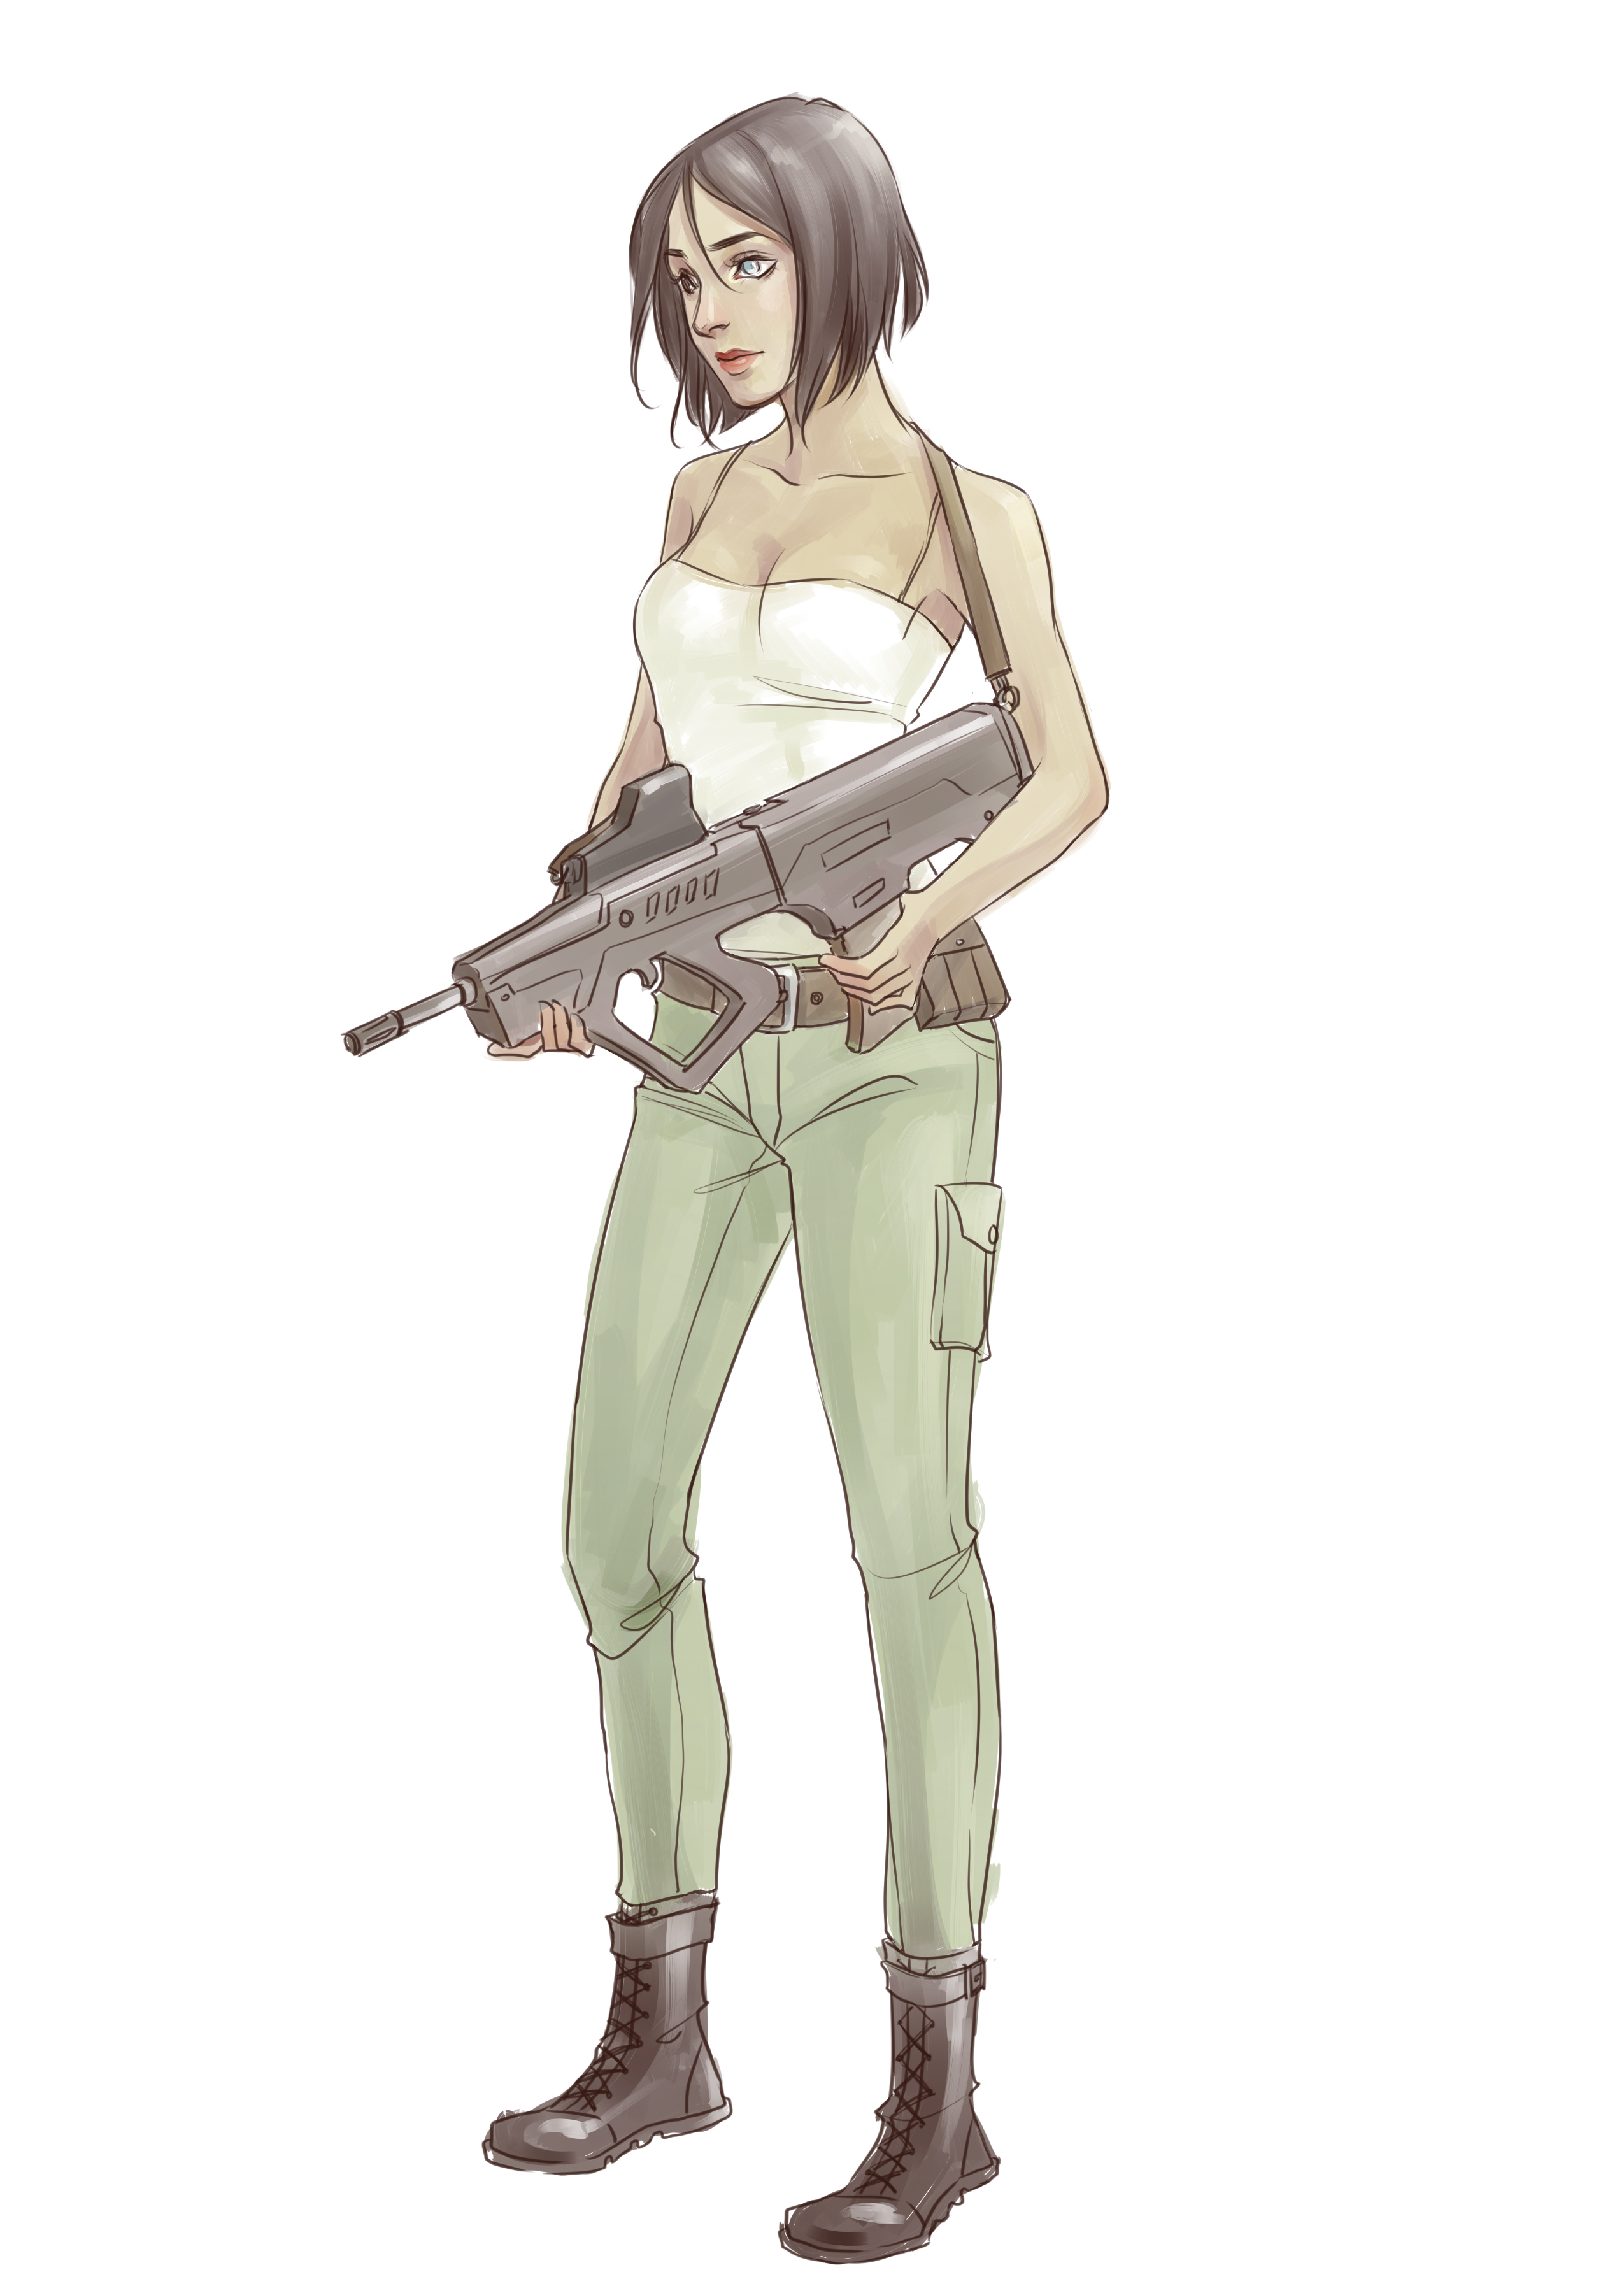
\includegraphics[width=12cm]{img/hayley.jpg}
\end{center}
